%\documentclass[preprint,10pt,authoryear]{elsarticle}

%% Use the option review to obtain double line spacing
%% \documentclass[preprint,review,12pt]{elsarticle}

%% Use the options 1p,twocolumn; 3p; 3p,twocolumn; 5p; or 5p,twocolumn
%% for a journal layout:
%% \documentclass[final,1p,times]{elsarticle}
%% \documentclass[final,1p,times,twocolumn]{elsarticle}
%% \documentclass[final,3p,times]{elsarticle}
%% \documentclass[final,3p,times,twocolumn]{elsarticle}
%% \documentclass[final,5p,times]{elsarticle}
%% \documentclass[final,5p,times,twocolumn]{elsarticle}

%% if you use PostScript figures in your article

%% or use the graphicx package for more complicated commands
\usepackage{graphicx}
%% or use the epsfig package if you prefer to use the old commands
\usepackage{epsfig}

%% The amssymb package provides various useful mathematical symbols
\usepackage{amssymb,amsmath}
%% The amsthm package provides extended theorem environments
%% \usepackage{amsthm}

%% The lineno packages adds line numbers. Start line numbering with
%% \begin{linenumbers}, end it with \end{linenumbers}. Or switch it on
%% for the whole article with \linenumbers after \end{frontmatter}.
\usepackage{lineno}

%% natbib.sty is loaded by default. However, natbib options can be
%% provided with \biboptions{...} command. Following options are
%% valid:

%%   round  -  round parentheses are used (default)
%%   square -  square brackets are used   [option]
%%   curly  -  curly braces are used      {option}
%%   angle  -  angle brackets are used    <option>
%%   semicolon  -  multiple citations separated by semi-colon
%%   colon  - same as semicolon, an earlier confusion
%%   comma  -  separated by comma
%%   numbers-  selects numerical citations
%%   super  -  numerical citations as superscripts
%%   sort   -  sorts multiple citations according to order in ref. list
%%   sort&compress   -  like sort, but also compresses numerical citations
%%   compress - compresses without sorting
%%
%% \biboptions{comma,round}

% \biboptions{}
\usepackage{hyperref}
\usepackage{color}
\usepackage{textcomp}
\usepackage{multirow}
\usepackage{float}
\usepackage{amsmath}

\journal{Computer and Chemical Engineering}

\begin{document}

\begin{frontmatter}
\title{Accelerating multi-dimensional population balance model simulations using GPU with a highly scalable framework.}


\author[label1]{Chaitanya Sampat}
\author[label1]{Yukteshwar Baranwal}
\address[label1]{Chemical and Biochemical Engineering, Rutgers University, Piscataway, NJ, USA - 08854}
\author[label1]{Rohit Ramachandran\corref{cor1}}
\ead{rohitrr@soemail.rutgers.com}
\cortext[cor1]{Corresponding author}
%\ead[url]{pslrutgers.com}

\begin{abstract}
Population Balance models are widely used in pharmaceutical industry to simulate
and optimize the granulation process.Prediction of the distribution of many 
particulate systems with the evolution of time using these models, has become an 
efficient tool for the on-line control of the granulation process. 
With increase in the number of components and phases in a particulate mixture, 
complexity of PBM increases. This leads to multi-dimensional matrix calculations 
requiring great computational power. Solving such a system with a traditional 
central processing unit (CPU) would be very time consuming, thus there is a 
need of a parallel framework which can help decrease the simulation time. 
Over the past decade, graphical process units (GPUs) are increasingly being 
used for computation. This study focuses on the development of an algorithm to 
parallelize the various nested loops inside the PBM. 
The PBM was developed for a continuous high shear granulation process and was made 
specifically for NVIDIA GPUs as it was developed on CUDA C/C++. The communication 
time is much lower in comparison to the speedup achieved in the parallel section 
of the code on the GPUs. The speed up achieved was significant compared to the PBM 
code when run in serial or in on multi-core configuration. The speed improvements 
for the code for various CPU \& GPU architectures and configurations have 
been reported. 
%The speed improvements were also tested with various combinations in 
%discretization of the granulator geometry and threads used for calculations. 
\end{abstract}

\begin{keyword}
%% keywords here, in the form: keyword \sep keyword
Population Balance Model \sep GPU \sep Parallel Computing \sep Granulation \sep MPI
%% MSC codes here, in the form: \MSC code \sep code
%% or \MSC[2008] code \sep code (2000 is the default)
\end{keyword}

\end{frontmatter}

\begin{linenumbers}
%% main text
\section{Introduction}
\label{secIntro}
Various chemical industries like detergent, food, pharmaceutical, fertilizers, catalyst encounter particulate processing daily. 
These processes constitute to about $50\%$ of the world's chemical production \citep{seville1997}.
In the pharmaceutical industry, particulate processes are widely used to increase 
the size of the granules, improve flow-ability, increase yield strength etc. One of 
major processes in among these to increase the granule size is granulation. 
Granulation is the process in which fine pharmaceutical powder 
blends are converted to larger granules using a liquid or a dry binder \citep{Chaturbedi2017}. 
These larger granules help in better flow ability and strength to these mixtures 
aiding further processing. 

%Due to the large number of collisions inside these systems, modeling these systems is a challenge.

Understanding the dynamics of the continuous granulating system is vital for its smooth 
operation and to reduce the amount of waste generated in the development phase. The Food 
and Drug administration (FDA) has also been promoting a similar initiative with its 
Quality by Design (QbD) and Process Analytically Tools (PAT) principles~\citep{sen2014}. 
Thus, a process model for the system becomes an integral part of the development phase. 
A model which predicts the bulk mechanical properties of the mixture as well as a particle size 
distribution (PSD) is required. Over the past decade, Population Balance Models (PBMs) have been used 
to predict the behavior of granulation processes \citep{Barrasso2013},\citep{Ramachandran2009}. 

PBMs are used to calculate bulk rate processes occurring during granulation. PBMs are sometimes 
unable to integrate certain information, thus a mechanistic kernel can be 
introduced in these models to make them more accurate. Another way to increase its accuracy, 
is to incorporate larger number of solid bins inside the PBM. The increase in the number of 
solid bins leads to an increase in calculations for each time step, leading to a higher 
simulation times. The calculations increase by a factor of $2^n$ where n being the number 
of solid bins. An accurate model which incorporates higher number of solid bins as well as 
includes a mechanistic kernel in its calculations is expected to be very 
slow to simulate and could take upto hours to complete. Such models and their solving 
techniques are not viable to be used in real time system control. Thus, there is a need to 
solve these models quicker.

The advancement of computers and its peripherals in recent years have led to a great increase in 
computational resources leading to faster simulations. The recent central processing unit (CPU) 
now contains various of cores thus making it possible to run multiples processes in parallel. 
In order to take advantage of a highly parallel framework, large number of cores are needed 
which may not be possible in a personal desktop and a supercomputer cluster needs to be used.
Another computer peripheral that can to be used to run a highly parallel code is the computer's 
graphic processing unit (GPU)~\citep{Prakash2013b}. These GPUs contain thousands of compute 
cores that can be used run tasks in parallel. Thus, a desktop equipped with a GPU could 
compute the same results as a CPU code on supercomputers in lesser amount of time as seen in Section \ref{secResults}.
With the launch of Compute Unified Device Architecture (CUDA), NVIDIA made it easier to use GPUs for 
general parallel programming in an approach usually termed as general purpose computing on GPUs (GPGPUs).

In the present study, a mechanistic multi-dimensional PBM was developed such that it was not 
only accurate but also scalable since the number of solid bins could be changed to alter its 
behaviour. This model was developed in C++ to be run on CPUs. This C++ model was parallelised 
using Message Parsing Interace (MPI) which is parallel application programming interface (API). 
This model was developed NVIDIA GPUs and was parallelized using the CUDA toolkit. The timings of 
the simulations were then compared for each of these cases. The scalability of the GPU based code 
was also tested to obtain speed improvements over serial CPU code.


\section{Background and previous works}
\label{secBkgd}
\subsection{Granulation and population balance modeling}
Granulation is the process of engineering granules from pharmaceutical powder blends 
with the addition of liquid or solid binders. This process is usually carried out 
to obtain granules with a certain PSD,  bulk densities and other physical properties~\citep{Barrasso2015cerd}.
There are about 3 rate processes that occur due the addition of a liquid binder to the 
powder mixture are wetting and nucleation, consolidation and aggregation, and breakage 
and attrition~\citep{sen2014}. In a high shear granulator, the particles are rendered wet 
when they come in contact with the liquid binder, which also aids in granule formation due to 
liquid bridges. These granules can also break into smaller fragments due to shear stresses, 
compressive and tensile forces that are exerted on to the system due the impeller, 
particle-particle interactions and particle-wall interactions.

To understand the process dynamics and control these process, population balance equations 
have been accepted as a relevant methodology \citep{Immanuel2005}. Population balances have been successful in 
predicting physical phenomena occurring in granulation such as aggregation, breakage and 
consolidation. These models predict how groups of distinct entities inside the pharmaceutical 
powder behave on a bulk scale due to process parameters over time of granulation. A
general representation of the model is:

\begin{align}
\frac{ \partial}{\partial t}&F(\textbf{v},\textbf{x},t) + \frac{\partial}{\partial 
\textbf{v}}[F(\textbf{v},\textbf{x},t)\frac{d\textbf{v}}{dt}(\textbf{v},\textbf{x},t)] 
+ \frac{\partial}{\partial \textbf{x}}[F(\textbf{v},\textbf{x},t)\frac{d\textbf{x}}{dt}
(\textbf{v},\textbf{x},t)] \notag\\
    &= 
\Re_{formation}(\textbf{v},\textbf{x},t)+\Re_{depletion}(\textbf{v},\textbf{x},t)
+\dot{F}_{in}(\textbf{v},\textbf{x},t) -\dot{F}_{out}(\textbf{v},\textbf{x},t) 
\label{eqn:bkgd_pbm_general} 
\end{align}

where $\textbf{v}$ is a vector of internal 
coordinates.  $\textbf{v}$ is commonly used to describe the solid, liquid, 
and gas content of each type of particle. The vector $\textbf{x}$ represents 
external coordinates, usually spatial variance. $F$ represents the 
number of particles present inside the system, $\dot{F}_{in}$ 
and $\dot{F}_{out}$ is the rate of particles coming in and going out the 
system respectively. $\Re_{formation}$ and $\Re_{depletion}$ are the rate of 
formation and depletion due various phenomena occurring in granulation. 

Prediction of PSDs and other particle bulk properties is highly dependent on 
the kernels used to describe the sub-processes inside granulation. Identification 
of a kernel that describes the sub-processes suitably is of the essence in this model 
since they are not only size dependent but also time dependent. Recently, various 
mechanistic kernels have been developed that help capture the micro-mechanics of the 
system, which help in better prediction of the final particle size \citep{Barrasso2015processes}. 
Several of these kernels maybe dependent on other physical simulations such as Discrete 
Element Model (DEM) to obtain certain information about the microscopic phenomena 
occurring inside the system.


\subsection{Parallel Computing}
Computing with its current infrastructure has become a very important tool in sciece. 
Parallel computing is one of most extensively used type of computing used by scientists 
to perform simulations. It is the process of splitting of larger calculations into 
many smaller processes executed concurrently \citep{Almasi1989}. This type of execution 
helps achieve large speed gains overs simulations run on a single core in a serial manner.
The computational task can be decomposed by various means to help simulate the system 
in a reasonable amount of time. The simulation problem can be decomposed either 
at the task level or at the data level. Task parallelism involves each process to 
behave distinctively from another as they would each be performing different operations. 
These multiple operations could be performed on a single data set or on multiple data 
sets, known as multiple instruction single data (MISD) and multiple instruction 
multiple data (MIMD) respectively. On the other hand, data parallelism 
involves the distribution of data across various processes which usually perform same set of 
operations on the data \citep{solihin2015}. This type of parallelism is also known 
as single instruction multiple data (SIMD). These two types of parallelism can also 
be combined in certain systems, thus decreasing the simulation times further.

\subsection{GPU based parallel computing}
Traditionally, large parallel jobs needed to be run on supercomputers which had thousands 
of cores, but these are require special components making them expensive.
Graphic processing unit (GPU) were initially mainly used for vector calculations to support 
graphics inside a computer system. But, lately GPU manufacturers have started to promote them 
general computing as well. This form of computing has been gaining popularity among scientists 
to accelerate simulations \citep{kandrot2011}. These GPUs dominantly have a 
massively parallel architecture with hundreds to thousands of computational cores 
which can thousands of active threads simultaneously \citep{keckler2011}. 
Modern GPU computing can be exploited using parallel programming languages 
such as OpenCL and CUDA. 

CUDA is an application programming interface (API) developed by NVIDIA \citep{NVIDIA2012} that enables 
users to program parallel code for execution on the GPU. This is framework is an 
extension implemented on top of C/C++ or Fortran. Parallel code for the GPU is written 
as kernels, which theoretically are similar to functions or methods in traditional 
programming languages. Only few sections of the code can be written in terms of kernel 
while the remaining has to be executed in serial on the CPU of the system. The \texttt{nvcc} 
compiler from the CUDA toolkit prioritizes the compilation of these kernels before 
passing the serial section of the code to the native C/C++ compiler inside the system. 
There are three main parallel abstractions that exist in CUDA are grids, blocks and 
threads \citep{santos2013}. Each CUDA kernel is executed serially during the execution 
of the program unless specified, where the kernels can be run in parallel using CUDA 
streams. Each kernel executes as a grid which in turn consists of various blocks which 
are consistuted by various threads. This thread-block-grid hierarchy helps obtain fine 
grained data level and thread level parallelism. An illustration of this hierarchy is 
observed in Figure \ref{fig:bkg_gpu_arch}.

Another important aspect related to GPU parallelization is the data communication between the threads. 
The GPU consists of various memory modules with different access limitations as shown in Figure 
\ref{fig:bkg_gpu_arch}. The threads inside each block can communicate with each other using the 
shared memory. This memory is local to the block where these threads exist i.e. they are not 
accessible by threads from other blocks. In addition to the shared memory each thread has its 
own local memory where local/temporary variables for each kernel can be saved to them. 
The threads from different communicate with each other using the global memory which is visible to 
all blocks inside the GPU at the cost of higher communication times. Accessing of data from the 
local memory is the fastest for a thread and its slows down as we move towards shared block memory 
and the least for accessing data from the global GPU memory. 


\begin{figure}
\centering
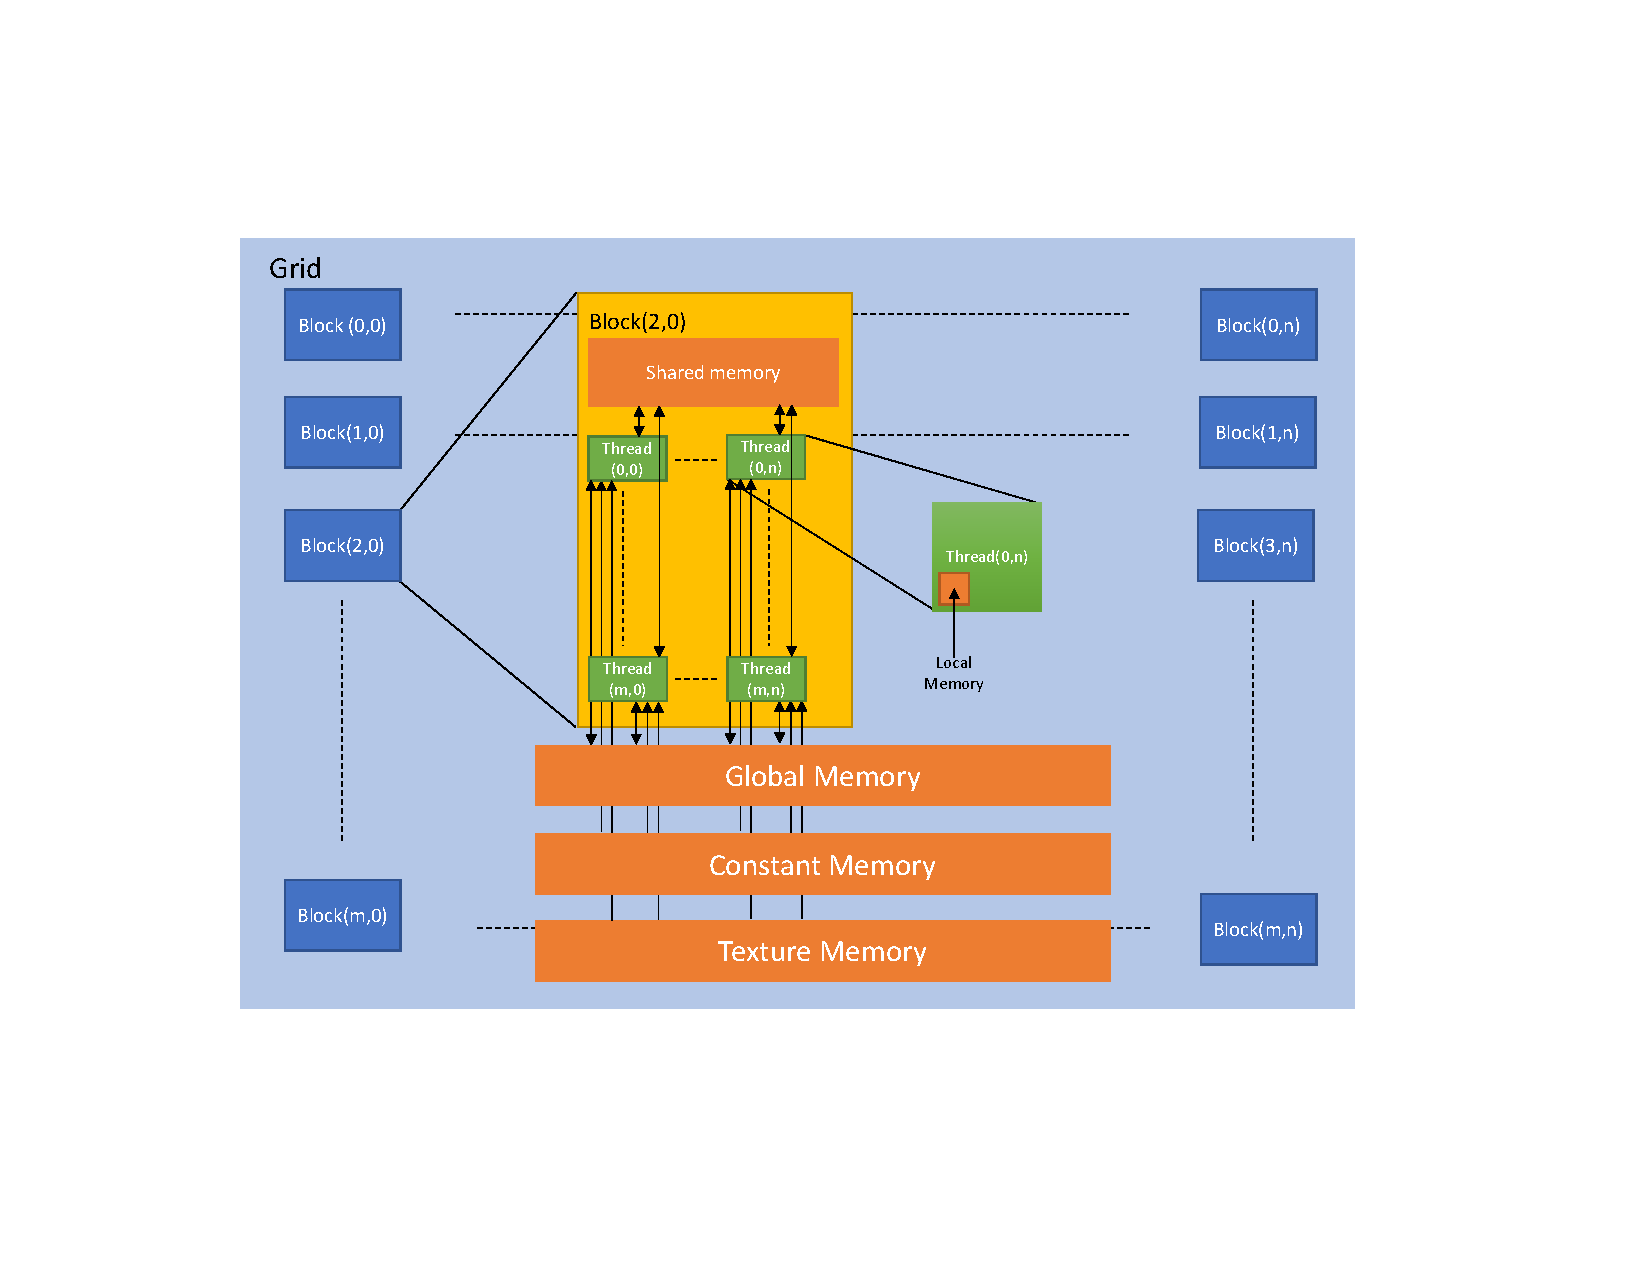
\includegraphics[scale=0.6]{bkg_gpu_arch.pdf}
\caption{The parallel structure matrix inside the GPU and the various memories associated 
with each structure.}
\label{fig:bkg_gpu_arch}
\end{figure}


\subsection{Previous parallel PBM works}
PBMs have known to be been computationally intensive especially ones with larger internal 
coordinates and higher dimensions. Thus, several researchers have made attempts to increase 
the speed of these simulations. \cite{Gunawan2008} developed a parallelization technique 
for a high-resolution finite volume solution of the PBM. The parallel algorithm presented by 
\cite{Gunawan2008} in their scale up studies for the PBM upto 100 cores achieved good 
parallel efficiency, implying the algorithm's effectiveness. The study was not performed for 
higher number of dimensions inside the PBM. This study also suggested that an algorithm 
with a shared memory model could help improve simulation speeds further. A hybrid memory model 
was implemented by \cite{Bettencourt2017} to obtain speed improvements of about 98\% from the 
serial code. This implementation took into account both Message Parsing Interface (MPI) as well 
as Open Multi-processing (OMP). A similar PBM parallelization approach was also undertaken in 
\citep{Sampat2018} and a speed up of about 13 was obtained. 

Algorithms to parallelize the PBM codes on GPU have been studied briefly by \cite{Prakash2013b} 
using the inbuilt MATLAB's parallel computing toolbox (PCT). This study was able to achieve 
good speed ups but could have been higher if the code had been implemented in native programming 
languages such as C or FORTRAN. Other works that have used GPU acceleration to improve computation 
times for their population balance simulations include those from various other chemical engineering 
processes such as crystallization \citep{Szilagy2016}, combustion \citep{Shi2012}, multiphase flow 
\citep{santos2013}, coagulation dynamics \citep{Xu2015}


\section{Method and implementation}
\label{secMethods}
\subsection{PBM implementation}
The population balance equation used in this work is expressed below:
\begin{align}
\frac{d}{dt}F(s_1,s_2,x)=\Re_{agg}(s_1,s_2,x)+\Re_{break}(s_1,s_2,x)+\dot{F}_{in}(s_1,s_2,x)-\dot{F}_{out}(s_1,s_2,x)
\label{eqn:mthds_pbm_overall} 
\end{align}
where, $F(s_1,s_2,x)$ is the number of particles with an active pharmaceutical ingredients (API) volume of $s_1$ and an excipient 
volume of $s_2$ in the spatial compartment $x$. The rate of change of number of particles with time 
in different size classes depend on the rate of aggregation $\Re_{agg}(s_1,s_2,x)$ and the rate of 
breakage $\Re_{break}(s_1,s_2,x)$. Also, the rate of particles coming into, $\dot{F}_{in}(s_1,s_2,x)$ and 
going out, $\dot{F}_{out}(s_1,s_2,x)$ of the spatial compartment due to particle transfer affect the number of 
particles in different size classes. 
The rate of change of liquid volume in each particle is calculated using the equation: 

\begin{align}
\frac{d}{dt}F(s_1,s_2,x)l(s_1,s_2,x)&= 
\Re_{liq,agg}(s_1,s_2,x)+\Re_{liq,break}(s_1,s_2,x)+\dot{F}_{in}(s_1,s_2,x)l_{in}(s_1,s_2,x)\notag\\
&-\dot{F}_{out}(s_1,s_2,x)l_{out}(s_1,s_2,x)+F(s_1,s_2,x)\dot{l}_{add}(s_1,s_2,x)
\label{eqn:mthds_pbm_rate} 
\end{align}

where, $l(s_1,s_2,x)$ is the amount of liquid volume in each particle with API volume of $s_1$ and 
excipient volume of $s_2$ in the spatial compartment $x$. $\Re_{liq,agg}(s_1,s_2,x)$ and 
$\Re_{liq,break}(s_1,s_2,x)$ are respectively the rates of liquid transferred between size classes due to 
aggregation and breakage. $l_{in}(s_1,s_2,x)$ and $l_{out}(s_1,s_2,x)$ are respectively the liquid 
volumes of the particles coming in and going out of the spatial compartment. $l_{add}(s_1,s_2,x)$ is 
the volume of liquid acquired by each particle in the compartment at every time step due to external 
liquid addition.
Similarly, the rate of change of gas volume is calculated using the following equation: 

\begin{align}
\frac{d}{dt}F(s_1,s_2,x)g(s_1,s_2,x)&= 
\Re_{gas,agg}(s_1,s_2,x)+\Re_{gas,break}(s_1,s_2,x)+\dot{F}_{in}(s_1,s_2,x)g_{in}(s_1,s_2,x)\notag\\
&-\dot{F}_{out}(s_1,s_2,x)g_{out}(s_1,s_2,x)+F(s_1,s_2,x)\dot{g}_{cons}(s_1,s_2,x)
\label{eqn:mthds_pbm_gas_agg} 
\end{align}

where, $g(s_1,s_2,x)$ is the gas volume of each particle with API volume of $s_1$ and excipient 
volume of $s_2$ in the spatial compartment $x$. $\Re_{gas,agg}(s_1,s_2,x)$ and 
$\Re_{gas,break}(s_1,s_2,x)$ are respectively the rates of gas transferred between size classes due to 
aggregation and breakage. $g_{in}(s_1,s_2,x)$ and $g_{out}(s_1,s_2,x)$ are respectively the gas 
volume of the particles entering and leaving the spatial compartment. $\dot{g}_{cons}(s_1,s_2,x)$ is the 
volume of gas coming out of each particle at every time-step due to consolidation of the particles. 
The rate of aggregation, $\Re_{agg}(s_1,s_2,x)$ in Equation \ref{eqn:mthds_pbm_overall} is 
calculated as: \citep{Chaturbedi2017}

\begin{align}
\Re_{agg}(s_1,s_2,x)&= \frac{1}{2}\int _0^{s_1} \int_0^{s_2} 
\beta(s_1',s_2',s_1-s_1',s_2-s_2',x)F(s_1',s_2',x)F(s_1-s_1',s_2-s_2',x)ds_1'ds_2'\notag\\ 
&- F(s_1,s_2,x)\int _0^{s_{max_1}-s_1} \int_0^{s_{max_2}-s_2} 
\beta(s_1,s_2,s_1',s_2',x)F(s_1',s_2',x)ds_1'ds_2'
\label{eqn:mthds_R_agg}
\end{align}


where, the aggregation kernel, $\beta(s_1,s_2, s_1',s_2',x)$ is expressed as a function of collision 
rate coefficient ($C$) and probability that collision results in agglomeration($\psi$) \citep{ingram2005}
and is shown below: 

\begin{align}
\beta(s_1,s_2,s_1',s_2',x) = \beta_oC(s_1,s_2,s_1',s_2',x)\psi(s_1,s_2,s_1',s_2',x)
%\beta(s_1,s_2,s_1',s_2',x) = & \beta_o*(V(s_1,s_2,x)+V(s_1',s_2',x))^{\gamma}*(c(s_1,s_2,x)\notag\\
%&+c(s_1',s_2',x))^{\alpha}\left(1-\frac{(c(s_1,s_2,x)+c(s_1',s_2',x))^{\delta}}{2}\right)^{\alpha}
\label{eqn:mthds_pbm_beta_kernal}
\end{align}

where, $\beta_o$ is aggregation rate constant.\\
Collision rate coefficient ($C$) is a function of particle sizes and is calculated by normalizing the 
number of collisions between group of particles \citep{gantt2006} and is obtained from LIGGGHTS 
DEM simulation. A recent study shows that collision frequency depends on PSD as well 
\citep{sen2014}. Collision rate coefficient can be expressed as:

\begin{align}
C(s_1,s_2,s_1',s_2')=\frac{N_{coll}(s_1,s_2,s_1',s_2')}{N_p(s_1,s_2)N_p(s_1',s_2')\Delta t}
\label{eqn:collfreq}
\end{align}

In Equation \ref{eqn:collfreq}, $N_{coll}$ is the number of collision between two particles in 
time interval $\Delta t$ \& $N_p$ is number of particle of particular size. The agglomeration 
($\psi$) in equation (\ref{eqn:mthds_pbm_beta_kernal}) can be expressed as:

\begin{align}
\psi((s_1,s_2,s_1',s_2') = 
\left\{\begin{matrix}
\psi_0,\hspace{0.2cm} LC((s_1,s_2) \geq LC_{min}\hspace{0.2cm} and\hspace{0.2cm} LC((s_1',s_2') \geq LC_{min}	\\ 
0,\hspace{0.2cm} LC((s_1,s_2) < LC_{min}\hspace{0.2cm} or\hspace{0.2cm} LC((s_1',s_2') < LC_{min}
\end{matrix}\right.
\label{eqn:colleff}
\end{align}
 In Equation \ref{eqn:colleff}, $LC$ is the liquid content of particles and $LC_{min}$ stands for minimum 
 liquid content required for coalescence of particles. 

%%%% commented the breakage details as we aren't including in results


Similarly, the breakage rate is expressed as-
\begin{align}
\Re_{break}(s_1,s_2,x) = \int_0^{s_{max_1}} \int_0^{s_{max_2}} 
K_{break}(s_1',s_2',x)F(s_1',s_2',x)ds_1'ds_2' - K_{break}(s_1,s_2,x)F(s_1,s_2,x)
\end{align}
	    
where, the breakage kernel $K_{break}(s_1,s_2,x)$ is formulated as: 

\begin{align}
K_{break}(s_1,s_2,x) = C_{impact}\int_{U_{break}}^{\infty}p(U)dU	    
K_{break}(s_1,s_2,x)=\left(\frac{4}{15\pi}\right)^{\frac{1}{2}}G_{shear}exp\left(-\frac{B}{R(s_1,s_2,x)}\right)
\end{align}


% where, $G_{shear}$ is the shear rate exerted by the impeller on the granules. $R(s_1,s_2,x)$ is 
the radius of the granule that breaks and $B$ is the breakage kernel constant. $G_shear$ is 
calculated as $\frac{\nu_{impeller}*D_{impeller}*PI}{60}$ where $\nu_{impeller}$ and $D_{impeller}$ 
are respectively the rotational speed and diameter of the impeller.
The rate of increase of liquid volume of a particle, $\dot{l}_{add}(s_1,s_2,x)$ is expressed as:

\begin{align}
\dot{l}_{add}(s_1,s_2,x) = \frac{(s_1+s_2)(\dot{m}_{spray}(1-c_{binder})-\dot{m}_{evap})}{m_{solid}(x)}
\label{eqn:mthds_liq_addn_rate}
\end{align}

where, $(s_1+s_2)$  is the total solid volume of the particle; $\dot{m}_spray$ is the rate of external 
liquid addition, $c_{binder}$ is the concentration of binder in the external liquid (which is assumed to 
be zero in this case); $\dot{m}_{evap}$ is the rate of evaporation of liquid from 
the system (which is also assumed to be zero in this case) and $m_{solid}$ is the total amount of solid 
present in the compartment.
The rate of decrease in gas volume per particle due to consolidation is calculated using the 
following expression: \citep{Verkoeijen2002} 

\begin{align}
\dot{g}_{cons}(s_1,s_2,x)=&c (\nu_{impeller})^{\omega}V(s_1,s_2,x)\frac{(1-\epsilon_{min})}{s} 
\notag \\ 
& \left[g(s_1,s_2,x)+l(s_1,s_2,x) -(s_1+s_2)\frac{\epsilon_{min}}{1-\epsilon_{min}}\right]
\label{eqn:mthds_rate_gas_vol_part}
\end{align}        

 where, $c$ and $\omega$ are the consolidation constants; $v_{impeller}$ is the impeller 
rotational speed; $V(s_1,s_2,x)$ is the volume of particle, $\epsilon_{min}$ is the minimum porosity; 
$g(s_1,s_2,x)$ and $l(s_1,s_2,x)$ are respectively the gas and liquid volumes of the particle.

 Particle transfer rate, $\dot{F}_{out}(s_1,s_2,x)$ in Equation \ref{eqn:mthds_pbm_overall} is calculated 
as:

\begin{align}
\dot{F}_{out}(s_1,s_2,x) = \dot{F}(s_1,s_2,x)\frac{\nu_{compartment}(x)*dt}{d_{compartment}}
\label{eqn:mthds_f_out_dot_part_trans_rate}
\end{align}

where, $\nu_{compartment}(x)$ and $d_{compartment}$ are respectively the average velocity of 
particles in compartment $x$ and the distance between the mid-points of two adjacent compartment, 
which is the distance particles have to travel to move to the next spatial compartment. $dt$ is the 
time-step.

\subsection{MPI implementation}
The message parsing interface (MPI) parallel implementation of the PBM was 
focused towards equal distribution of the task and memory. The implementation 
used in this work differs from the hybrid implementation used by \citep{Bettencourt2017}
and \citep{Sampat2018} since only MPI was used to parallelize the code. It 
was pointed by \citep{Sampat2018} that open message parsing (OMP) does not 
provide significant speed improvements due to limitations with usage of 
dynamic vectors which are essential for such a system. Thus, the OMP 
implementation was avoided which also meant that lesser number of cores 
would be required to run the code. As the work is mainly focused on using 
desktop computers over supercomputers, it meant that most of these studies 
could be performed on personal computer. These simulations were performed 
on a computer with an Intel Core i7-7700K processor clocked at 4.2GHz and 
32 GB of RAM. For maximum performance while data reading and writing a SSD 
was used. GCC version 7.4 with openMPI 2.0 was used to compile 
the parallel C++ code.





To obtain the most optimal parallel performance, when solving the PBM, workloads 
were distributed in a manner which took into account the shared and‎ distributed 
memory aspects of the clusters, the PBM was being run on. To parallelize the model 
in a way which could take advantage of shared memory but still effectively run 
across a distributed system both MPI and OMP were implemented. One MPI process 
was used per CPU core and one‎ OMP thread was used per CPU core, as 
Bettencourt et al. (2017) found it resulted in the best‎ performance. MPI was 
used for message passing from one node to another while OMP was used‎ for 
calculations on each node that could be efficiently solved using a shared 
memory system.‎ An algorithm in the form of pseudo code is presented in the 
Appendix illustrating how the calculations‎ are distributed and carried out 
during the simulation. For each time step, the MPI processes are‎ made 
responsible for a specific chunk of the spatial compartments. Then each 
OMP thread, inside‎ of each MPI process, is allocated to one of the cores 
of multi-core CPU the MPI process is bound‎ too. The OMP threads divide up 
and compute $R_agg$. After $R_agg$ is calculated the MPI processes‎ calculate 
the new PSD value for their chunk at that specific time step, Ft,c. The 
slave processes‎ send their Ftc to the master processes which collects them 
into the complete Ft,all. The master‎ process then broadcasts the Ft, all 
value to all slave processes. This decomposition of the data into‎ 
different CPUs and further into various threads is illustrated in 
Figure 3-4.‎ A crucial feature of the PBM is that the current PSD (Ft,all) 
value is used to compute a new‎ time step size for the next iteration. 
This means all of the MPI processes need to have the same‎ dynamic time 
step size at each iteration for the calculations to be properly carried 
out in parallel.‎ Since the completely updated Ft, all value is shared 
before calculating a new time step each process‎ will have the same Ft, 
all value. As a result each process calculates the same size for the 
new time‎ step.‎ Since the DEM informed PBM code required dynamic size 
increase for the data structure due‎ to different number of particles 
being present in the DEM simulation, the PBM code developed‎ used the 
Standard Template Library containers and their features available 
in C++ 11 and later.‎ It requires intel v17.0.2 (GCC 5.3+) or later 
for compilation. Since this module was not present on‎ the Stampede,
the execution of the PBM was done on the newer Stampede2 supercomputer. 
Each‎ of the compute node of the cluster consists of Intel Xeon Phi 7250 
(“Knights Landing") which has‎ 68 cores on a single socket clocked at 1.4 GHz, 
with 96 GB of DDR4 RAM. Each of the cores‎ consists of 4 hardware threads. 
The simulations were then run by varying the number of MPI‎ processes from 
1 to 16 and the number of OMP threads from 1 to 8, thus, using a maximum of 128‎ cores.

\subsection{GPU implementation}
NVIDIA’s CUDA toolkit extends the C language such that user defined functions 
called kernels can be created to be run on the GPU. These kernels can be 
executed N times in parallel using large number of threads. A thread is 
sequence if programmed instructions that can be managed by the computer’s 
scheduler. A kernel depending upon the dimensions of the data can execute 
instructions in 1-D, 2-D or 3-D thread blocks. The kernel can also launch 
multiple thread blocks at once, thus increasing the number of parallel 
process executions known as grid. Similar to a thread block, a grid can 
be up to 3-D depending upon the data under study.
The code execution was split between the CPU (also called host) and GPU 
(also called device). Time sensitive calculations as well as mixed data 
calculations were handled on the CPU with a single core, while the more 
computationally intensive tasks were distributed on to the GPU using 
kernels. Like in the CPU parallelization, the geometry was split into 
multiple compartments. These compartments in turn formed the number of 
blocks inside each GPU kernel. The number of solids used helped formed 
the threads in each of these blocks. The work flow of the execution can 
be found in Figure 3-5. The orange arrows in Figure 3-5 indicate the 
transfer of data from the CPU memory to the GPU memory and vice-versa 
whereas the blue arrows indicate the sections of the code that is sent 
to the GPU for parallel execution.

\begin{figure}
\centering
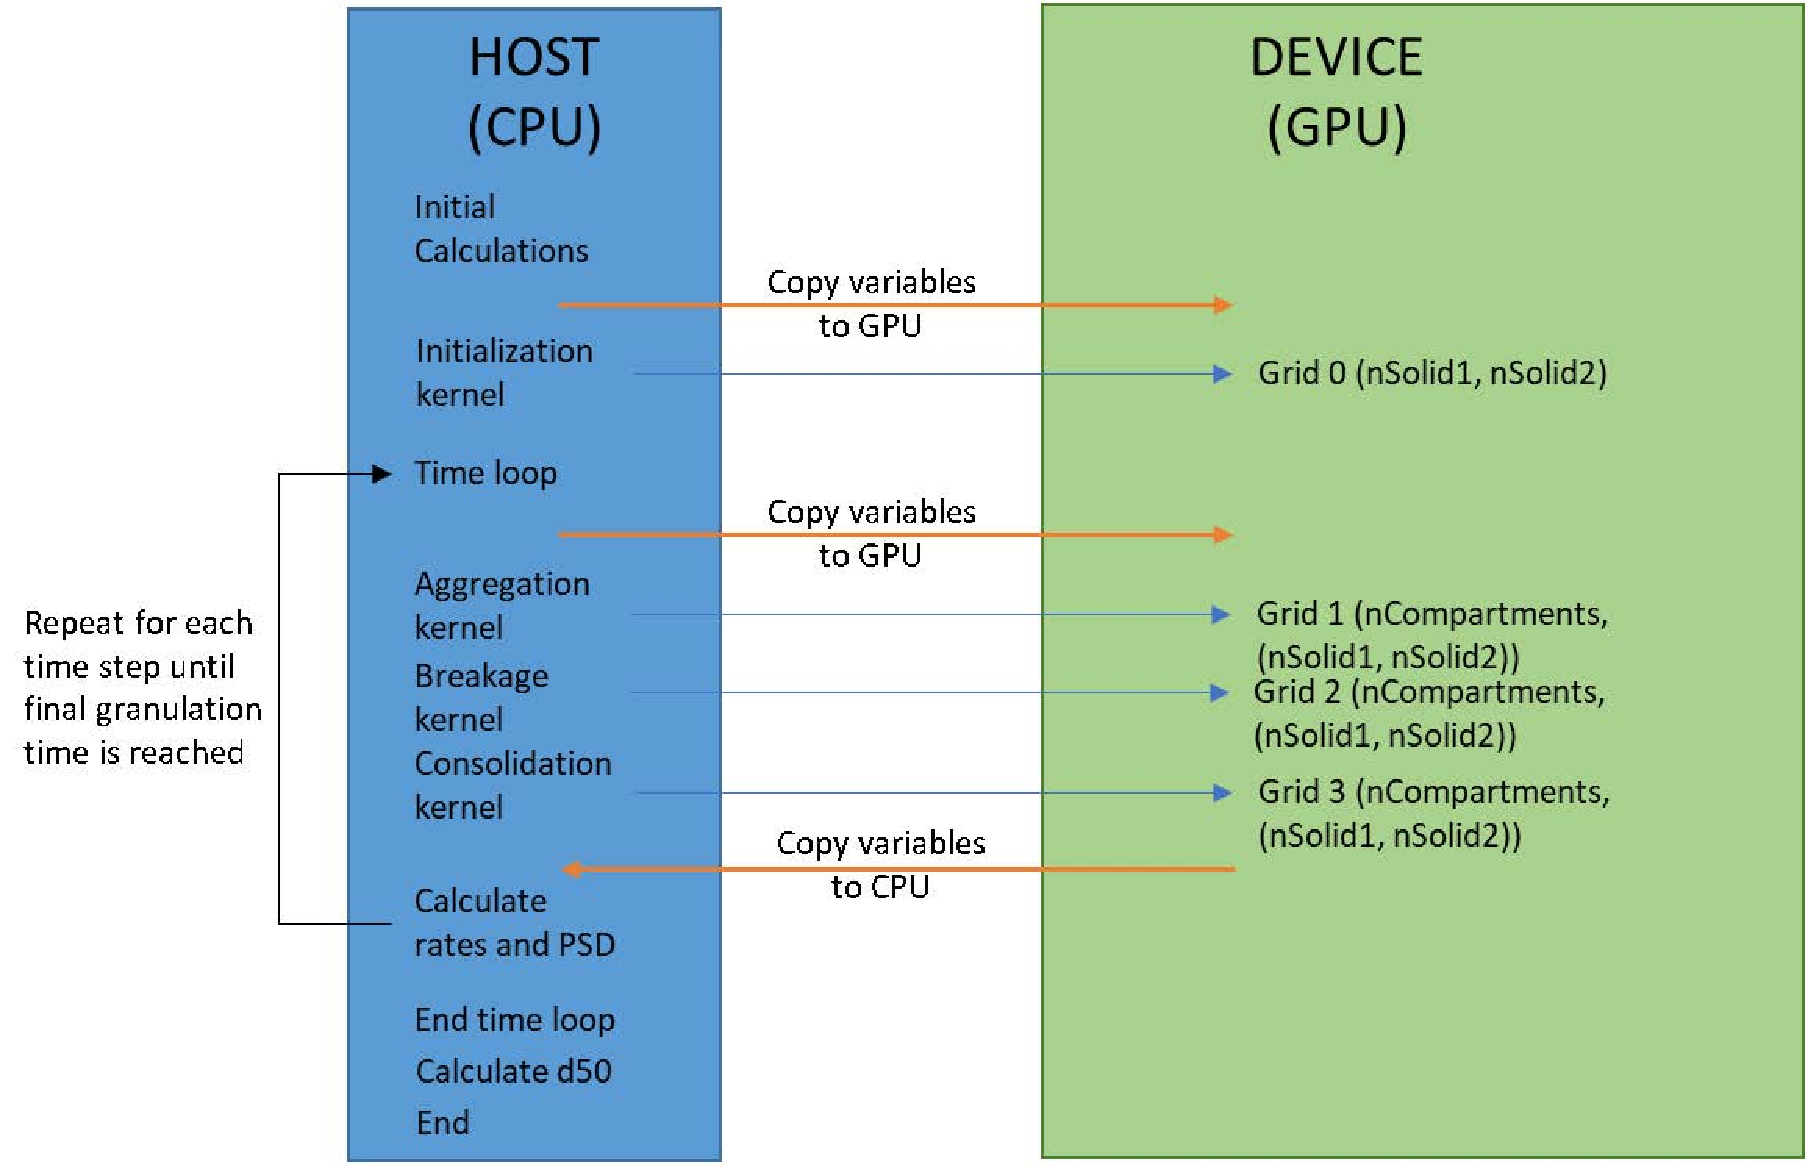
\includegraphics[scale=0.4]{gpuImp_schematic.pdf}
\caption{Workflow of the GPU code indicating data transfers and execution timeline of the code.}
\label{fig:mtd_gpu_imp}
\end{figure}

\section{Results and discussions}
\label{secResults}S
\subsection{GPU performance}
Talk about code performance first and then about the profile of the code
The GPU parallel code timings were not compared directly to the CPU 
version since it would have been unfair since the hardware configurations 
used were completely different. There are several non-code related latency 
and delays that could affect the performance of the code. Thus, no 
comparison was performed between the 2 code versions. 
A soft scaling was performed for the GPU code. This refers to change of 
the size of the problem is in direct correlation with the computational 
power required for its execution. In this study, the sections of geometry 
were varied from 2 to 16 compartments, while the number of solids from 1 
to 16 for both the solids. Using this configuration, the maximum number 
of threads required would be 4096 while the minimum would be 2 threads. 
Figure 4-7 shows timing comparison between the studies. It can be seen 
that as the size of the problem increases there is a small increase in 
the time of the simulation which can directly be linked to increase in 
the number of calculations as well problem initiation times would be 
higher. A larger time is required for problems which require threads 
greater than the number of CUDA cores present on the GPU (here 1792), 
since the extra blocks would need to wait for the earlier blocks to 
complete their simulations before they can be executed.

\subsection{Performance on GPUs compared to CPUs}

\subsection{Server level GPU code performance}



I still need to figure out some studies to complete this section.

\section{Conclusions}
\label{secConc}
\end{linenumbers}

\bibliographystyle{elsarticle-harv}
\bibliography{pbmGpuPaper}


\end{document}

%%
%% End of file `elsarticle-template-num.tex'.
